\documentclass[journal]{IEEEtran}

\ifCLASSINFOpdf
\else
\fi

% correct bad hyphenation here
\hyphenation{op-tical net-works semi-conduc-tor}
\usepackage[british]{babel}
\usepackage[hidelinks, unicode]{hyperref}
\usepackage[utf8]{inputenc}
\usepackage[T1]{fontenc}
\usepackage{amsmath}
\usepackage{bm}
\usepackage{amsfonts}
\usepackage{tabularx}
\usepackage{float}
\usepackage{mathtools,amsthm}
\usepackage{supertabular}
\usepackage{array}
\usepackage{multirow}
\usepackage{graphicx}
\usepackage[flushleft]{threeparttable}
\graphicspath{ {./images/} }

\usepackage[capitalize, nameinlink, noabbrev]{cleveref}

\begin{document}

\title{\vspace{-0.5em}Small Nucleolar RNAs in breast cancer\\[0.1em]\huge \textit{Project report}}
\author{\href{https://github.com/bocchilorenzo}{Lorenzo Bocchi}, \href{https://github.com/valefras}{Valentino Frasnelli}, \href{https://github.com/erich-r}{Erich Robbi}, \href{https://github.com/annalisaxamin}{Annalisa Xamin} \vspace{0.25cm}\\\ \textit{Laboratory of Biological Data Mining}\\ Department of Information Engineering and Computer Science\\University of Trento, Italy\\

\normalsize\{\href{mailto:lorenzo.bocchi@studenti.unitn.it}{\texttt{lorenzo.bocchi}},  \href{mailto:valentino.frasnelli@studenti.unitn.it}{\texttt{valentino.frasnelli}}, \href{mailto:erich.robbi@studenti.unitn.it}{\texttt{erich.robbi}},  \href{mailto:annalisa.xamin@studenti.unitn.it}{\texttt{annalisa.xamin}}\} \texttt{@studenti.unitn.it}\vspace{-1em}}%


\maketitle
%----------------------------------------------------------------------------------
%\small{\tableofcontents}

\begin{abstract}
The canonical roles of small nucleolar RNAs (snoRNAs), which include ribosome biogenesis and RNA modification, are well recognized. snoRNAs function as endogenous sponges that control the expression of miRNAs. Therefore, accurate snoRNA expression is essential for adjusting miRNA expression. Similarly to miRNAs, snoRNAs that have been converted into miRNA-like sequences are essential to control the expression of protein-coding genes. SnoRNA dysregulation is related to breast cancer (BC), according to recent findings. By allowing breast cells to develop cancer hallmarks, the inappropriate expression of snoRNA leads to the pathogenesis of breast cancer.
This study tries to validate any causal association between snoRNA and breast cancer using quantitative methodologies such as machine learning-based approaches, statistical testing, and descriptive statistics.
Furthermore, a study of the network of gene expansions conducted on FANTOM5, a dataset that is used as a reference for physiological conditions for the human body, will be conducted.
\end{abstract}

% Note that keywords are not normally used for peer-review papers.
\begin{IEEEkeywords}
snoRNA, small nucleolar RNA, human tissues, RNA-Seq, snoRNA/host gene relationship,  transcriptome, ribosome, regulation.
\end{IEEEkeywords}


\IEEEpeerreviewmaketitle

\section{Introduction}
%\subsection{Context}
\IEEEPARstart{S}{mall} nucleolar RNAs (snoRNAs) are a conserved type of noncoding RNA, best characterized for their role in ribosome biogenesis\cite{Zhang2019}. 
The three main categories of classic snoRNAs are as follows: first, the C/D box snoRNAs (\textbf{SNORDs}), which are typically 60 to 90 nucleotides long and contain C/D box motifs (C: RUGAUGA and D: CUGA). Next, the H/ACA box snoRNAs (\textbf{SNORAs}) have H/ACA box motifs (H: ANANNA and ACA: ACA) and range in length from 120 to 140 nt. Third, the size of small Cajal body-specific RNAs (\textbf{SCARNAs}) varies substantially, and they contain different combinations of the C/D and H/ACA motifs. SCARNAs are localized to Cajal bodies, where it is hypothesized that they contribute to the modification of U1 to U6, while the SNORDs and SNORAs normally reside in the nucleolus where they are incorporated into RNPs that change rRNA. \cite{vanderWerf2021} \newline

Because of recombination and retrotransposition from an ancestral snoRNA, many snoRNAs exist in mammalian genomes in multiple copies. They are encoded either in the intronic region of the larger host gene or independently outside the gene and are highly distributed in the nucleolus of eukaryotic cells. In particular, Box C/D snoRNA family members are frequently encoded in the same host gene, whereas box H/ACA family members typically occur in many hosts. Moreover, the regulation of snoRNAs encoded in the same host gene can differ depending on the tissue, as does the quantity of some snoRNAs within the same family \cite{Bergeron2021}. These non-coding RNAs play a key roles in the RNA modification process: they function as guide RNAs for the site-specific modification of target RNAs such as rRNAs and snRNAs \cite{Yoshihama2013} (\cref{fig:functions_snoRNAs} reports a detailed description of all their functions). \newline

\begin{figure}[h]
    \centering
    \includegraphics[width=0.5\textwidth]{images/Functions_snoRNAs.png}
    \caption{\textbf{Function of snoRNAs}. \textbf{A}. snoRNAs are derived from the snoRNA genes with independent promoters, or intronic snoRNA genes encode them. \textbf{B}. The canonical function of snoRNAs is realized by guiding 2'-O-methylation and pseudouridylation of rRNAs in the nucleolus. \textbf{C}. scaRNAs also guide 2'-O-ribosemethylated nucleotides and pseudouridines on snRNAs in cajal bodies. \textbf{D}. The "orphan" snoRNAs play an important role in alternative splicing. \textbf{E}. snoRNAs bind to PARP1 and stimulate its catalytic activity to promote rDNA transcription. \textbf{F}. snoRNAs are also enriched in chromatin, which suggests a chromatin-associated role. \textbf{G}. snoRNAs can be processed into sno-derived RNA (sdRNA), which has been shown to perform a regulatory function similar to microRNAs. snoRNA= small nuclear RNA. \newline
    Reprinted from \textit{Small nucleolar RNA is potential as a novel player in leukemogenesis and clinical application}, by L. M. Lin, Q. Pan, Y. M. Sun, and W. T. Wang, Blood Science, vol. 3, no. 4, pp. 122–131, Oct. 2021 \cite{Lin2021}.}
    \label{fig:functions_snoRNAs}
\end{figure}

%\subsection{Problem definition}
Previous research has shown that snoRNAs, which are primarily thought to be housekeeping genes, influence rRNA synthesis. However, this assumption has recently been questioned. Through signaling pathways and cell cycles, snoRNAs may have an impact on the control of tumor cell growth and death. 
Gene amplification and gene inhibition may dramatically alter a person's genetic makeup by encouraging cancer development. Therefore, understanding the mechanisms underlying genes whose expression is altered or enhanced will help us to understand how cancers arise and progress. In particular, snoRNA's expression appears to be dysregulated in a peculiar way, indicating that the incidence of cancer is intimately associated with these dysregulations. \cite{Zhang2019} \newline

For this reason, the issues that this project tries to address are whether there is a difference in the level of expression of snoRNAs in our genes of interest in the presence of breast cancer compared to healthy individuals. \newline
Recent research highlighted the role of some host genes in the presence of cancer, where changes in snoRNA expression were analyzed and genes such as \emph{GAS5} and \emph{ZFAS1} were found to have important functions in cancer development, acting, respectively, as regulators of cell death and proliferation and tumour suppressive ncRNA\cite{Williams2012}. \newline

%\subsection*{Purpose Formalization}
The key point of this project is to compile a list of potential genes that could be relevant for breast cancer and to analyze their expression levels in cancer patients compared to the control group, which in our case is made up of healthy patients.
In addition, our objective is to find if there are causal relationships between snoRNAs and genes linked to breast cancer and if there are differences in the expression levels of those genes between the control and treatment groups.

\section{Materials and methods}
The pipeline of the project, as illustrated in \cref{fig:pipeline}, consists of applying the RMA normalization to a Gene Expression Omnibus data set. After that, a subset of the gene of interest is gained and on that, a feature selection is applied. Then, we continued with the differential expression analysis and model tuning and fitting. 
We also performed network analysis using gene network expansions from the FANTOM5 dataset.

\subsection{Data preprocessing}
The very first step is to collect data.
For what concerns, the gene expansion and network analysis data from the FANTOM5 project\cite{Lizio2015} have been used.
The Fantom dataset has been created with the CAGE technology, which identifies all the transcriptional starting sites (TSS) for a gene. \newline
%For this reason, 181 genes correspond to more than 181 gene isoforms, but this will be reviewed more in depth further on in the report. 
The snoDB 2.0 database\cite{Bergeron2022} has also been used to match information. After collecting the datasets, the relevant genes are extracted from FANTOM5 and joined with those from snoDB. 
%This is a single \textit{csv} file that contains all relevant snoRNAs and information about their host genes.

The resulting dataset is then filtered once again to only keep snoRNAs and host genes that, according to research, play a role in the development of breast cancer. In particular, the snoRNAs kept are:
\begin{table}[h!]
    \centering
    \begin{tabularx}{\linewidth}{| X | X | X |}
        \hline
        SNORA1 & SNORA12 & SNORA14B \\ \hline
        SNORA16A & SNORA21 & SNORA23 \\ \hline
        SNORA24 & SNORA32 & SNORA38 \\ \hline
        SNORA44 & SNORA48 & SNORA49 \\ \hline
        SNORA52 & SNORA53 & SNORA57 \\ \hline
        SNORA61 & SNORA63 & SNORA64 \\ \hline
        SNORA65 & SNORA70 & SNORA71C \\ \hline
        SNORA73A & SNORA73B & SNORA75 \\ \hline
        SNORA78 & SNORA8 & SNORD10 \\ \hline
        SNORD102 & SNORD104 & SNORD105 \\ \hline
        SNORD105B & SNORD108 & SNORD110 \\ \hline
        SNORD111B & SNORD113-3 & SNORD113-4 \\ \hline
        SNORD114-1 & SNORD114-13 & SNORD114-14 \\ \hline
        SNORD114-19 & SNORD114-20 & SNORD114-21 \\ \hline
        SNORD115-23 & SNORD115-32 & SNORD116-13 \\ \hline
        SNORD119 & SNORD12 & SNORD12B \\ \hline
        SNORD13 & SNORD14A & SNORD14C \\ \hline
        SNORD14D & SNORD15B & SNORD16 \\ \hline
        SNORD17 & SNORD18A & SNORD1B \\ \hline
        SNORD20 & SNORD22 & SNORD26 \\ \hline
        SNORD28 & SNORD29 & SNORD32A \\ \hline
        SNORD33 & SNORD34 & SNORD35A \\ \hline
        SNORD36A & SNORD36B & SNORD38A \\ \hline
        SNORD3A & SNORD3D & SNORD41 \\ \hline
        SNORD42A & SNORD42B & SNORD44 \\ \hline
        SNORD45A & SNORD47 & SNORD49B \\ \hline
        SNORD4B & SNORD5 & SNORD50A \\ \hline
        SNORD52 & SNORD53 & SNORD54 \\ \hline
        SNORD55 & SNORD56 & SNORD57 \\ \hline
        SNORD58A & SNORD58C & SNORD59A \\ \hline
        SNORD60 & SNORD63 & SNORD64 \\ \hline
        SNORD65 & SNORD68 & SNORD69 \\ \hline
        SNORD71 & SNORD74 & SNORD76 \\ \hline
        SNORD8 & SNORD81 & SNORD82 \\ \hline
        SNORD84 & SNORD86 & SNORD87 \\ \hline
        SNORD89 & SNORD94 & SNORD96A \\ \hline
        SNORD97 & SNORD99 & \\ \hline
    \end{tabularx}
    \caption{List of snoRNAs involved in the development of breast cancer (according to literature).}\label{table:snoRNAs_list}
\end{table}
\newpage
And their host genes:
\begin{table}[h!]
    \centering
    \begin{tabularx}{\linewidth}{| X | X | X |}
        \hline
        TMX1 & ZFAS1 & CDKN2B-AS1 \\ \hline
        CWF19L1 & EIF4A1 & EP400 \\ \hline
        HIF1A-AS2 & MEG8 & NOP56 \\ \hline
        RACK1 & RPL13A & RPS13 \\ \hline
        SCARNA12 & SNHG12 & SNHG20 \\ \hline
        SNHG5 & SNHG6 & SNHG7 \\ \hline
        SNHG8 & AP1G1 & CFDP1 \\ \hline
        CHD8 & DDX39B & EEF2 \\ \hline
        EIF4A2 & EIF4G2 & GAS5 \\ \hline
        GNL3 & HSPA8 & HSPA9 \\ \hline
        IPO7 & MYRIP & NAN \\ \hline
        NCL & NFATC3 & PCAT4 \\ \hline
        PPAN & PRKAA1 & PRRC2A \\ \hline
        PTCD3 & RABGGTB & RNF149 \\ \hline
        RPL10 & RPL12 & RPL13 \\ \hline
        RPL17 & RPL21 & RPL23 \\ \hline
        RPL23A & RPL4 & RPL7A \\ \hline
        RPLP2 & RPS11 & RPS2 \\ \hline
        RPS20 & RPS3 & RPS8 \\ \hline
        SF3B3 & SLC25A3 & SNHG1 \\ \hline
        SNHG3 & SNHG9 & SNORD1C \\ \hline
        SNORD35B & SNORD37 & SNRPB \\ \hline
        SNX5 & TAF1D & TNPO2 \\ \hline
        TOMM20 & WDR43 & \\ \hline
    \end{tabularx}
\caption{List of host genes}\label{table:host_genes_list}
\end{table}

\begin{figure}[H]
    \centering
    \includegraphics[width=\linewidth]{images/flowchart.jpg}
    \caption{Project pipeline}\label{fig:pipeline}
\end{figure}

For the rest of the analysis, two datasets from Gene Expression Omnibus (GEO) have been used. In particular, firstly, we tried our pipeline by merging the following datasets from GEO: \href{https://www.ncbi.nlm.nih.gov/geo/query/acc.cgi?acc=GSE10810}{GSE10810}\cite{pedraza2010gene}, \href{https://www.ncbi.nlm.nih.gov/geo/query/acc.cgi?acc=GSE29431}{GSE29431}\cite{lopez2012biomedical}, \href{https://www.ncbi.nlm.nih.gov/geo/query/acc.cgi?acc=GSE42568}{GSE42568}\cite{clarke2013correlating} and \href{https://www.ncbi.nlm.nih.gov/geo/query/acc.cgi?acc=GSE61304}{GSE61304}\cite{aswad2015genome}. After a first try, we decided to continue our work with a different dataset, but still about breast cancer patients: \href{https://www.ncbi.nlm.nih.gov/geo/query/acc.cgi?acc=GSE45827}{GSE45827}\cite{Gruosso2016}.\newline
The first GEO dataset used contains both control and test samples: in particular, it contains expression data of the genes both in presence of cancer and in healthy patients. It was obtained from a combination of different data sets, all related to breast cancer: GSE10810 (58 samples), GSE29431 (66 samples), GSE42568 (121 samples), and GSE61304 (62 samples). They all contain the same genes and their combination amounts to a total of 307 samples, 60 of which are control samples with no breast cancer. The data was created using an Affymetrix Human Genome U133 Plus 2.0 Array.
Later, prompted by some issues with the data which will be discussed in the results section, we decided to use the data coming from the Gene Expression Omnibus with id GSE45827\footnote{\url{https://www.ncbi.nlm.nih.gov/geo/query/acc.cgi?acc=GSE45827}}. This dataset contains 178 samples of "Expression data from Breast cancer subtypes" coming from 155 different patients. This data was also created with the same Affymetrix Human Genome U133 Plus 2.0 Array platform. \newline

To prepare the data for analysis, we follow the following steps:
\begin{enumerate}
    \item We loaded the data with the \textit{affy} library\cite{Gautier2004} in R.
    \item We proceeded with a normalization step to remove batch effects from the Affymetrix arrays data. On the raw micro-array data we used the RMA (Robust Multiarray Analysis)\cite{Irizarry2003} normalization. In this way, probes that mapped to the same gene have been collapsed to one computing average for the gene expression value.
    \item The logarithmic value of all gene expression levels was calculated and used downstream in the analysis.
    \item Transpose the matrix and add columns useful for ML prediction (such as the binary predictor variable for the absence or presence of cancer in the first dataset or the multiclass predictor variable in the second dataset for the cancer subtypes).
\end{enumerate}

Why did we need to perform a normalization?

Affymetrix GeneChips are made up of a number of probes, each designed to measure the expression levels of a particular genomic sequence. Each probe consists of hundreds of short 25-mer oligonucleotide strands that match the target mRNA sequence exactly. RNA samples are transformed into cRNA (complimentary RNA) using an in vitro transcription method that. cRNA is fragmented, biotin labels are attached, and the fragments are washed over the chip. cRNA fragments hybridise with their respective oliginucleotide sequence, resulting in an increase in abundance of biotinylated cRNA molecules on the probe. A fluorescent dye is washed over the chip and binds to the biotin labels. A fluorescent scan of the chip gives fluorescence values for each probe, which are directly related to the abundance of cRNA fragments hybridised to the probe. These fluorescence levels can be used to infer the relative abundance of specific mRNA sequences in a sample, giving a "snapshot" of the transcriptome.

Affymetrix Genechips are designed in such a way that each gene is matched to 11-20 such probes evenly distributed throughout the chip. These probes make up a Probe Set on the chip. The presence of noise is a large problem in large scale microarray studies, and can come from a number of sources. Noise due to non-specific binding of cRNA fragments to probes is one such source, and is eleviated through the use of probes on the chip designed to measure for non-specific binding. Each probe described above, termed a Perfect Match probe (PM) is matched to a second probe, termed a Mis-Match probe (MM). MM probes are identical to PM probes but for the middle (13th) nucleotide in the sequence, which is replaced with it's complement. By subtracting the signal for the MM probe from the signal for the PM probe, a value for the true signal is reached.

However, it has been shown that the signal strength for the MM probes can often be larger than that of the PM probes, implying that the MM probe detects both the true signal and background signal. This can result in non-sensical negative expression values. RMA is a normalisation procedure for microarrays that background corrects, normalises and summarises the probe level information without the use of the information obtained in the MM probes \cite{Irizarry2003, Irizarry2003b, Bolstad2003}.

\subsection{Exploratory Data Analysis}
EDA is a way of analyzing data sets to summarize their essential properties, frequently utilizing statistical graphics and other data visualization approaches. There are several techniques available for EDA; in our work, we used Principal Component Analysis.

PCA consists in projecting orthogonally a dataset $X = x_1 , \dots , x_n$ of $n$ $p$-dimensional points into a $r$-dimensional space with $r = min(n-1,p)$, so that in the new coordinates the projected points’ variables are uncorrelated.
The new coordinates are called principal components, and each component is defined by the rules:
\begin{itemize}
    \item being orthogonal to the previous components 
    \item having highest possible variance
\end{itemize}

The first principal component corresponds to a line that passes through the multidimensional mean and minimizes the sum of squares of the distances of the points from the line. Each eigenvalue is proportional to the portion of the “variance” (more correctly of the sum of the squared distances of the points from their multidimensional mean) that is associated with each eigenvector.
The sum of all the eigenvalues is equal to the sum of the squared distances of the points from their multidimensional mean The explained variance of $k_{th}$ principal component is is $\lambda_k / \sum_i \lambda_i$. PCA essentially rotates the set of points around their mean in order to align them with the principal components. This moves as much of the variance as possible (using an orthogonal transformation) into the first few dimensions.

\subsection{Differential gene expression analysis}
After having removed the batch effect, we proceeded to find differentially expressed genes or (DEGs). It's important to note that this procedure was done only on the second dataset.

Differential Gene Expression analysis refers to the analysis and interpretation of differences in abundance of gene transcripts within a transcriptome \cite{CHEN2019324}. Practically, it consists of normalizing the read count data and performing a hypothesis test for the means, to observe quantifiable differences in expression levels between the groups.

DGE analysis in this case is performed in order to assess the difference between control and treatment. More specifically, the difference between the control and the different cancer subtypes.
To perform this analysis, we used the \textit{limma} package of R \cite{Ritchie2015}.

\subsection{Feature selection}
The best way to proceed would be by carrying out a feature selection on our data, firstly, by removing all the genes that are not relevant to the project, afterwards, we further reduce the number of features via an algorithmic selection.

To do so, we fit a regularized algorithm, called LASSO, which applies a penalty to the coefficients in order to introduce bias in the model. This penalty makes it so that the coefficients can decrease to zero, performing feature selection in an embedded way. By tuning the penalty through cross-validation, the variables can be subset to an acceptable number, allowing us to fit the models without worrying about the $p>>n$ problem. Furthermore, the coefficients with the optimal penalty can provide us with further insight into how correlation in gene expression is related to the presence of breast cancer.

\subsection{Classification models}
Fitting a classification model with our gene expression data will allow us to infer useful information and assess whether it is possible to perform a classification that predicts our cancer subtype groups with the transcripts of the genes we have chosen.

The models we are fitting and testing on our data are:
\begin{itemize}
    \item Logistic regression
    \item Lasso
    \item Random forest
    \item Support vector machine (more specifically kernel machines)
\end{itemize}

The choice of such models was justified by some of their embedded properties. Logistic regression, like LASSO, outputs coefficients and significance (p-value) for each variable, which once again can give us insight into how gene expression correlates with the presence or absence of breast cancer.
On the other hand, random forest computes variable importance, which can be useful to extract more insight from our data.
Support vector machines were chosen for being largely considered the best performing ML classifier, and in this project, they are used to understand just how good the classification performance can get.\newline
Now, a brief theoretical introduction to the various classification methods.

\subsubsection{Logistic regression}
Logistic regression models the probability of an event taking place by having the log-odds of such event be the linear combination of the covariates:
\begin{equation*}
ln(\frac{p}{1-p}) = \beta_0 + \beta_1\times X_1 + \ldots + \beta_k\times K_k
\end{equation*}
The logistic function then converts such log-odds to a value between 0 and 1 through the logistic function, so that one has the probability of a sample to belong to a certain class. The coefficients of the logistic regression are calculated by maxmimum-likelihood estimation, finding the best $\beta_k$ values by optimizing the fit on the log-odds. These coefficients are important for analysis, since they tell how a variable varies when the dependent variable (response) varies. 


\subsubsection{Lasso}
Lasso (Least absolute shrinkage and selection operator) is a regression method that performs variable selection through regularization to improve the prediction accuracy and interpretability of the resulting statistical model. The aforementioned regularization occurs in the form of shrinkage, implemented through a penalty applied to the coefficients, which, in the particular case of Lasso, shrinks coefficients in order to introduce bias and decrease the variance in the best fit model, restricting the influence of the predictors. Not only does such penalty shrink coefficients towards zero, but it also makes them zero, making the model sparse (some of the variables do not influence the outcome) and therefore simpler. This can be seen as a form of variable selection, ideal for the domain of the project, where most likely we will have to deal with large amounts of variables and a selection of them will be necessary. Of course, coefficients, which have not shrunk to zero are useful for interpretability of the model, giving more insight into the roles of the variables.\newline
Now, Lasso penalty is usually used in linear regression models, which are not suited for our purpose, since the project will most likely deal with classification problems, not regression ones. Fortunately, the Lasso regularization technique is easily extended to so-called Generalized Linear Models, a more general and flexible formulation of linear regression, which allows to use shrinkage in a classification context, and more specifically in a logistic regression model.

\subsubsection{Random forest}
Random forest is an ensemble Machine Learning algorithm. For classification, it works by creating $N$ classification trees and taking the most recurring response class predicted by the trees. It uses the bootstrap method, meaning that for each tree it creates a training set composed of randomly selected samples to avoid always fitting the same data on all the trees. Also, when building these decision trees, each time a split in a tree is considered, a random sample of $m$ predictors is chosen as split candidates from the full set of $p$ predictors. The split is allowed to use only one of those $m$ predictors. A fresh sample of $m$ predictors is taken at each split, and typically we choose $m \approx \sqrt{p}$. The reason for this is that in the dataset there might be a very strong predictor. This means that most if not all of the trees in the ensemble would use this predictor, making all the trees very similar and possibly highly correlated. Averaging many correlated trees have a smaller reduction in variance than averaging uncorrelated trees; therefore, we force each split to only consider a random subset of the possible predictors.

\subsubsection{Support vector machines}
Support Vector Machines, for short SVMs, are another supervised ML algorithm that can be used for classification. More specifically, they are divided in three subclasses:
\begin{itemize}
    \item Hard Margin Classifiers
    \item Soft Margin SVMs
    \item Non-linear SVMs
\end{itemize}
The first subclass, Hard Margin Classifiers (also called Maximal Margin Classifiers), represents the simplest form of SVM. The idea is that, given a set of $n$ labelled and linearly separable samples, there is a hyperplane that can separate the examples. But this does not give a single solution since, therefore we choose the one that maximizes the margin between the two classes. The margin is 2 * the smallest distance of any point to the hyperplane. If such a solution exists, the algorithm is guaranteed to find the globally optimal solution. The samples that “sit” on the margin are called Support Vectors, and they are the only ones that matter to the final boundary. Finding the maximal margin requires solving a constrained optimization problem via quadratic programming. The major issue with this subclass of SVMs is that it only works with linearly separable problems with no chance of misclassification. This means that even if the data are generally linearly separable, but there is a single misclassified example, there will not be a solution.
To overcome this, we move to the second subclass, Soft Margin SVMs.

The key difference between Soft Margin SVMs and Hard Margin SVMs is that here we introduce the concept of slack variables $\varepsilon$. A slack variable $\varepsilon_i$ measures the penalty for example $x_i$ for not satisfying the margin constraint. In particular, based on its value we can assert where the sample is located with respect to the hyperplane:
\begin{itemize}
    \item $\varepsilon_i = 0 \rightarrow $ the sample is on the correct side of the hyperplane and does not violate the margin
    \item $0 < \varepsilon_i < 1 \rightarrow $ the sample is on the correct side of the hyperplane but violated the margin
    \item $\varepsilon_i = 1 \rightarrow $ the sample is on the hyperplane and cannot be classified
    \item $\varepsilon_i > 1 \rightarrow $ the sample is on the wrong side of the hyperplane and it’s misclassified
\end{itemize}
The sum of all slack variables is minimized in the objective of the SVM together to the inverse margin and it’s multiplied to a parameter C. This parameter allows a trade off between data fitting and misclassifications. The higher its value, the more misclassifications are allowed. If it’s 0, we simply have a Hard Margin Classifier.

What if we have a non-linearly separable problem? In that case we can resort to the third subclass of SVMs, Non Linear SVMs. The idea is that we can define a higher dimensional space with respect to the one the data is in with p* > p dimensions (p is the number of dimensions in the original space) and then perform linear classification in this higher dimensional space. We can do so by mapping the features in the higher dimensional feature space. An example of mapping is the polynomial mapping which maps features to all possible conjunctions of features of a certain degree d (in case of the homogeneous mapping). One issue with this approach is that computation can be highly expensive in very high dimensions. We can use a trick called “kernel trick” which uses a kernel function that acts as a dot product in some p* dimensional space for some mapping. The most common kernel functions are:
%controllare qui sotto se le formule son giuste
%avevo corretto alcuni pezzi perché erano cannati ma non ho più riguardato
\begin{itemize}
    \item linear kernel $= K(x, z) = x \cdot z = \sum_{j=1}^{p} x_j z_j  $ non linear SVMs in this case coincide with Soft Margin SVMs
    \item polynomial kernel $ = K(x, z) = (1 + \sum_{j=1}^{p} x_j z_j)^{m}$ adds a constant to the linear kernel and gets elevated to a certain degree (with m = 2 one obtains a second degree kernel for example)
    \item radial kernel $= K(x, z) = exp(-\gamma \sum_{j=1}^{p} (x_j - z_j)^{2})$ with $\gamma > 0$ here the kernel tends to 0 the further x gets from z
\end{itemize}
Once again, we need to cross validate to understand which kernel to use and which parameters are best.

To be sure that the models actually yield relevant results, not only cross validation is applied but also a fit on 'housekeeping genes' and low variable genes is performed and compared with the fit on our genes of interest. The selected housekeeping genes are described in \Cref{table:housekeeping_genes_list}.
\begin{table}[h!]
    \centering
    \begin{tabularx}{\linewidth}{| X |  X |}
        \hline
        \textbf{Gene symbol} &  \textbf{Gene description} \\ \hline \hline
        C1orf43 & Chromosome 1 open reading frame 43 \\ \hline
        CHMP2A & Charged multivesicular body protein 2A\\ \hline
        EMC7  & ER membrane protein complex subunit 7\\ \hline
        GPI & Glucose-6-phosphate isomerase \\ \hline
        PSMB2 & Proteasome subunit, beta type, 2 \\ \hline
        PSMB4 & Proteasome subunit, beta type, 4\\ \hline
        RAB7A & Member RAS oncogene family \\ \hline
        REEP5 & Receptor accessory protein 5 \\ \hline
        SNRPD3 & Small nuclear ribonucleoprotein D3 \\ \hline
        VCP & Valosin containing protein \\ \hline
        VPS29 & Vacuolar protein sorting 29 homolog \\ \hline
        ACTG1 & Cytoskeletal Gamma-Actin \\ \hline
        RPS18 & Ribosomal Protein S18  \\ \hline
        POM121C & POM121 Transmembrane Nucleoporin C  \\ \hline
        MRPL18 & Mitochondrial ribosomal protein L18  \\ \hline
        TOMM5 & Translocase of outer mitochondrial membrane 5  \\ \hline
        YTHDF1 & YTH N6-methyladenosine RNA binding protein 1  \\ \hline
        TPT1 & Tumor protein, translationally-controlled 1\\ \hline
        RPS27 & Ribosomal protein S27\\ \hline
    \end{tabularx}
\caption{List of housekeeping genes}\label{table:housekeeping_genes_list}
\end{table}

Housekeeping genes are genes that are involved in basic cell maintenance and, therefore, are expected to maintain constant expression levels in all cells and conditions. Their identification facilitates exposure to the underlying cellular infrastructure and increases understanding of various structural genomic features. In addition, they are instrumental for calibration in many biotechnological applications and genomic studies. So, we have chosen the gene listed above as control as suggested from the literature\cite{Eisenberg2013, Caracausi2017} because they are expected to be expressed in all cells of an organism under normal conditions, irrespective of tissue type, developmental stage, cell cycle state, or external signal.
Subsequentally, \Cref{table:low_var_predictors} illustrates genes with few alterations in their expression levels in the dataset.

\begin{table}[h!]
    \centering
    \begin{tabularx}{\linewidth}{| X | X | X |}
        \hline
        LINC00189 & SCEL  & CDH7 \\ \hline
        FAM9B & NAALAD2 & GRTP1-AS1 \\ \hline
        DCAF4L2 & LINC02059 & LINC00408 \\ \hline
        UST-AS1 & PRKCA-AS1 & PHLDB2 \\ \hline
        LINC00301 & LINC01020 & TYR \\ \hline
        FMR1NB & C4orf33 & DNAH6 \\ \hline
        C11orf87 & GATM & SLC9C2 \\ \hline
        PCDHGB7 & HISLA & CNOT6L \\ \hline
        CFAP97 & LHFPL3-AS1 & ARPP21 \\ \hline
        MPP4 & CDC14C & LINC01990 \\ \hline
        UBDP1 & BCL2L14 & LINC01692 \\ \hline
        PPP4R3C & LINC02297 & HNF4A-AS1 \\ \hline
        CAGE1 & LARGE-AS1 & PKIA-AS1 \\ \hline
        MYLK3 & LIFR-AS1 & SAMMSON \\ \hline
        LINC02395 & BDNF-AS & LINC00102 \\ \hline
        SLC17A1 & IGF2BP2-AS1 & TRAV36DV7 \\ \hline
        BRPF3-AS1 & LMOD3 & LINC02424 \\ \hline
        GRK4 & MIPOL1 & F11 \\ \hline
        TRAF3IP2-AS1 & LINC01088 & EAF2 \\ \hline
        ZNF605 & GSK3B-DT & WARS2-AS1 \\ \hline
        ALDOB & DAZ4 & DAZ3 \\ \hline
        DAZ1 & DAZ2 & GYPA \\ \hline
        PDE6C & DHFRP3 & SLC13A1 \\ \hline
        MCFD2P1 & KRTAP9-9 & WNT16 \\ \hline
        ZFY & DEFB126 & CDH26 \\ \hline
        CABS1 & LINC02555 & LINC02619\\ \hline
         LINC00644 & ASB5 & MMAA \\ \hline
         TECRL & VWC2 & ADAM30 \\ \hline
    \end{tabularx}
\caption{List of low variable genes}\label{table:low_var_predictors}
\end{table}

\subsection{Network analysis}
Finally, we perform a network analysis on the FANTOM5 dataset using only the genes that we are interested in. This allows us to understand all possible interactions among genes related to a particular network. Therefore, we are able to find causal relationships among our genes of interest using OneGene, a method that uses PC-algorithm. We run this method on the BOINC platform in order to expand our list of genes, thanks to the computational power provided by gene@home volunteers. To represent the interactions that resulted from the expansions, we decided to build a network representing the connections among the genes. To do this, a fork of the library Tools\_Expand\_Genes\_Network\footnote{\url{https://github.com/gabrieletome/Tools_Expand_Genes_Network}} was created and made available on Github\footnote{\url{https://github.com/bocchilorenzo/Tools_Expand_Genes_Network}}. The reason for this was that the original library does not plot the nodes with the name of the gene, but with a number. This is not useful for the purpose of this project and, therefore, the library was edited to plot the gene names instead.

The input to the library is a zip file containing all the various gene isoforms downloaded from gene@home. These isoforms are themselves zip files that contain a .expansion and a .interaction file. The library then proceeds to build a complete graph of interaction and find an LGN of the genes. The local gene network is discovered using an adapted version of the Charikar algorithm \cite{10.5555/646688.702972}.

Before explaining the results obtained with each method, we briefly introduce a few key concepts.

\subsubsection{PC-algorithm}
The PC-algorithm is a method that allows estimating the equivalence class for a high-dimensional directed acyclic graph (DAG). It starts from a complete, undirected graph and recursively deletes edges based on conditional independence decisions. This yields an undirected graph that can be partially directed and further extended to represent the underlying DAG. This algorithm runs in the worst case in exponential time, but if the true underlying DAG is sparse, it is reduced to a polynomial runtime. This can be achieved by reducing the search space from the individual DAGs to equivalence classes. Therefore, the focus is on estimating the equivalence class and the skeleton of DAGs corresponding to multivariate Gaussian distributions in a high-dimensional context, or where the number of nodes $p$ may be much larger than the sample size $n$.
Generally, the PC-algorithm is divided in two steps:
\begin{itemize}
    \item creation of the skeleton of the DAG;
    \item extension of the skeleton to the equivalence class.
\end{itemize}
There are two main versions of the skeleton creation:
\begin{itemize}
    \item population version = perfect knowledge about all necessary conditional independence relations is assumed available
    \item sample version = the nodes correspond to multivariate normal distributed random variables, and thus it uses partial correlations to approximate conditional independencies
\end{itemize}
Usually, the exact conditional independence relations are not known, therefore it is better to consider the sample version. Partial correlations are computed via regression or other methods; for each result, it is possible to define a two-sided statistical test, where the null hypothesis is "partial correlation of nodes $i$ and $j$ given a set of nodes $k$ is 0", with a significance level $\alpha$ (the only tuning parameter). In case of the gene@home project, linear correlations are computed using the Pearson coefficient:

\begin{equation*}
  r = \frac{\sum_{i=1}^{n}(x_i-\bar{x})(y_i-\bar{y})}{\sqrt{\sum_{i=1}^{n}(x_i-\bar{x})^2}\sqrt{\sum_{i=1}^{n}(y_i-\bar{y})^2}}
\end{equation*}
The steps to assign direction to some of the edges of the graph are:
\begin{itemize}
    \item Given any pair of non-adjacent variables $i$ and $j$ with common neighbour $k$, orient $i - k - j$ into $i \rightarrow k \leftarrow j $if $k$ is not in $S(i, j)$ (which is the separation set computed during skeleton construction)
    \item Orient $j - k$ into $j \rightarrow k$ whenever there is an arrow $i \rightarrow j$ such that $i$ and $k$ are nonadjacent
    \item Orient $i - j$ into $i \rightarrow j$ whenever there is a chain $i \rightarrow k \rightarrow j$
    \item Orient $i - j$ into $i \rightarrow j$ whenever there are two chains $i - k - j$ and $i - l - j$ such that $k$ and $l$ are nonadjacent
    \item Orient $i - j$ into $i \rightarrow j$ whenever there are two chains $i - k - l$ and $k - l - j$ such that $k$ and $l$ are nonadjacent
\end{itemize}
There are some variants to this algorithm, namely:
\begin{itemize}
    \item PC-Stable Algorithm (PC*): the deletion of an edge takes place after all sizes of the neighborhood have been tested, leading to more conditional independence tests overall, but the result is independent from the order of the operations. This gives the ability to parallelize the computation, using the GPU and speeding up the process
    \item PC-Iterative Method (PC-IM) = the algorithm is performed iteratively on tiles, subsets of variables each of which contains all the variables already known to belong to some network to expand, plus some other variables chosen at random
\end{itemize}
OneGene uses the second variant, the PC-Iterative Method.

\subsubsection{OneGene}
OneGene is an algorithm that is used to perform gene network expansion. It was developed as a successor to $\text{NES}^{2}\text{RA}$ with the objective of reducing the delay between the user query and the response from the system. The inputs to the algorithm are:
\begin{itemize}
    \item set of transcripts and an expression matrix with the expression levels of each transcript in various conditions;
    \item tuple of parameters, those being set of alpha values, set of subset size and set of number of iterations;
    \item local gene network (LGN) to expand.
\end{itemize}
The OneGene pipeline is divided in two steps:
\begin{itemize}
    \item \textbf{pre-computation}: for each transcript in the set, multiple PC-IM iterations are performed. A single of those iterations corresponds to a $\text{NES}^{2}\text{RA}$ run with the single transcripts as LGN and the probability usually set to always 1. The result is the candidate expansions list for the transcript with all the parameters. There is no aggregation here and the expansions are stored for later use;
    \item \textbf{real-time interaction}: when all transcripts belonging to the desired LGN have been expanded, OneGene aggregates the results using different ranking aggregators. The aggregated result is given back to the user.
\end{itemize}

\subsubsection{Network Validation}
The approach to validate the network was to extract from snoDB all the snoRNAs in our selection, extract their target genes when available and check in our network how many of the snoRna - target connections were satisfied. In total, 231 snoRna - target connections were gathered, with 60 snoRNAs that had no recorded targets in snoDB, namely:
\begin{center}
    \tablefirsthead{\hline}
    \tablelasttail{\hline}
    \bottomcaption{List of snoRNAs with no target on snoDB}
    \begin{supertabular}{ |l|l|l| }
        SNORD14A & SNORD8 & SNORD32A \\
        SNORD14C & SNORD58C & SNORA71C \\
        SNORD36B & SNORD55 & SNORA8 \\
        SNORD4B & SNORD5 & SNORD33 \\
        SNORD71 & SNORA12 & SNORD86 \\
        SNORD99 & SNORA64 & SNORD68 \\
        SNORD18A & SNORD45A & SNORD37 \\
        SNORD97 & SNORA53 & SNORA57 \\
        SNORD58A & SNORD35B & SNORA48 \\
        SNORD36A & SNORD111B & SNORA49 \\
        SNORD14D & SNORD26 & SNORA52 \\
        SNORD42B & SNORA61 & SNORD65 \\
        SNORA24 & SNORA23 & SNORD102 \\
        SNORD57 & SNORD110 & SNORD87 \\
        SNORD96A & SNORD69 & SNORD54 \\
        SNORD17 & SNORA38 & SNORA1 \\
        SNORD3A & SNORD74 & SNORD1C \\
        SNORD44 & SNORD29 & SNORA63 \\
        SNORD49B & SNORD36C & SNORA16A \\
        SNORD58B & SNORD34 & SNORA32 \\
    \end{supertabular}
\end{center}

\section{Results and Discussion}
\subsection{First part: initial dataset and suspicious results}
Analyzing the data raises some issues. In particular, plotting X and Y the results are unexpected and seemingly wrong. As we can see in figures \ref{fig:resfitold},\ref{fig:reslevold} and \ref{fig:scalelocold} the plots have strange patterns that should not appear. This sort of strange issue is confirmed by trying to fit the models.

Trying this technique with a Random Forest yields suspicious results. Fit on genes of interest:
\begin{table}[!ht]
    \centering
    \begin{tabular}{cc|cc}
    \multicolumn{2}{c}{}
        & \multicolumn{2}{c}{Truth} \\
        & & No Cancer & Cancer\\ 
        \cline{2-4}
        \multirow{2}{*}{\rotatebox[origin=c]{90}{Predicted}}
        & No Cancer & 12 & 0 \\
        & Cancer & 3 & 62 \\ 
        \cline{2-4} \\ \\
    \end{tabular}
    \caption{Random forest fit on our genes of interest (old data)} \label{Table:fit_goi1}
\end{table}

\begin{table}[!ht]
    \centering
    \begin{tabular}{c|cccc}
    \multicolumn{1}{c}{} \\ 
        & Accuracy & Precision & Recall & F1 \\ 
        \cline{1-5}
        No Cancer & 0.9615 & 1 & 0.80 & 0.89 \\
        Cancer & 0.9615 & 0.95 & 1 & 0.98 \\ 
        \hline \\ 
    \end{tabular}
    \caption{Random forest performance measures on our genes of interest (old data)} \label{Table:fit_goi2}
\end{table}

The fit on housekeeping genes can be seen in \cref{Table:fit_house1} and its performance measures in \cref{Table:fit_house2}.
\begin{table}[!ht]
    \centering
    \begin{tabular}{cc|cc}
    \multicolumn{2}{c}{}
        & \multicolumn{2}{c}{Truth} \\
        & & No Cancer & Cancer\\ 
        \cline{2-4}
        \multirow{2}{*}{\rotatebox[origin=c]{90}{Predicted}}
        & No Cancer & 9 & 0 \\
        & Cancer & 6 & 62 \\ 
        \cline{2-4} \\ \\
    \end{tabular}
    \caption{Random forest fit on housekeeping genes (old data)} \label{Table:fit_house1}
\end{table}
\begin{table}[!ht]
    \centering
    \begin{tabular}{c|cccc}
    \multicolumn{1}{c}{} \\ 
        & Accuracy & Precision & Recall & F1 \\ 
        \cline{1-5}
        No Cancer & 0.9221 & 1 & 0.60 & 0.75 \\
        Cancer & 0.9221 & 0.91 & 1 & 0.95 \\ 
        \hline \\
    \end{tabular}
    \caption{Random forest performance measures on housekeeping genes (old data)} \label{Table:fit_house2}
\end{table}

This issue with regards to the dataset drove the group to try and find another set of data to use, possibly more accurate.

\subsection{Second part: new dataset}
The decision was to use the data from the Gene Expression Omnibus with id GSE45827\footnote{\url{https://www.ncbi.nlm.nih.gov/geo/query/acc.cgi?acc=GSE45827}}. This dataset contains 178 samples of expression data from Breast cancer subtypes coming from 155 different patients. This data was also created with the same Affymetrix Human Genome U133 Plus 2.0 Array platform.
Additionally, this new dataset is stratified differently with respect to the previous one, as the variable containing the condition of the patient is not binary as before, but instead is divided in 5 levels that correspond to different breast cancer subtypes:
\begin{itemize}
    \item 0 Normal (no cancer)
    \item 1 Basal 
    \item 2 Her2
    \item 3 Luminal A
    \item 4 Luminal B
\end{itemize}
The analysis of the new data yields significantly better results. The first model to fit was a Random Forest on the genes of interest, with the following performances during cross validation (best to worst):
\begin{table}[!ht]
    \begin{threeparttable}
    \centering
        \begin{tabularx}{\linewidth}{ X | X | X | X | X }
            \hline
            \textbf{mtry*} &
            \textbf{Measure} &  \textbf{Mean} & \textbf{N. folds} & \textbf{Std. error} \\ \hline
            10 & F1 & 0.7872726 & 5 & 0.03857438 \\
            22 & F1 & 0.7630541 & 5 & 0.03922816 \\
            16 & F1 & 0.7593441 & 5 & 0.04674310 \\
            28 & F1 & 0.7388160 & 5 & 0.04477342 \\
            58 & F1 & 0.7301482 & 5 & 0.04794219 \\
        \end{tabularx}
        \begin{tablenotes}
            \item *mtry is the number of predictors used for the splits
        \end{tablenotes}
     \end{threeparttable}
\end{table}

Testing the model against the test set yields the following confusion matrix:
\begin{table}[!ht]
    \centering
    \begin{tabular}{cc|ccccc}
    \multicolumn{2}{c}{}
        & \multicolumn{5}{c}{Truth} \\
        & & Basal & HER & L. A & L. B & Normal\\ 
        \cline{2-7}
        \multirow{5}{*}{\rotatebox[origin=c]{90}{Predicted}}
        & Basal & 9 & 2 & 0 & 1 & 0 \\
        & HER & 2 & 5 & 0 & 1 & 0 \\ 
        & L. A & 0 & 1 & 6 & 2 & 0 \\ 
        & L. B & 0 & 0 & 1 & 4 & 0 \\ 
        & Normal & 0 & 0 & 0 & 0 & 1 \\ 
        \cline{2-7} \\
    \end{tabular}
\end{table}

From the matrix we can extract an overall accuracy of 71.43\% and the following measures:
\begin{table}[H]
    \centering
    \begin{tabular}{c|cccc}
    \multicolumn{1}{c}{} \\ 
        & Accuracy & Precision & Recall & F1 \\ 
        \cline{1-5}
        Basal & 0.8571 & 0.75 & 0.82 & 0.78 \\
        HER & 0.8286 & 0.63 & 0.63 & 0.63 \\ 
        L. A & 0.8857 & 0.67 & 0.86 & 0.75 \\ 
        L. B & 0.8833 & 0.60 & 0.75 & 0.67 \\ 
        Normal & 1 & 1 & 1 & 1 \\ 
        \hline \\
    \end{tabular}
\end{table}\label{}
When extracting the variable importance from the model, seen in \cref{fig:vip_rf_interest}, it is interesting to notice that SNORD50B and its host gene SNHG5 are in the top 10 most important genes for classification.
%perché è interessante? che rilevanza ha? è uno sno particolare?

\noindent Fitting the model with only the lesser variant genes, the performance drops, as can be seen from the cross validation data:
\begin{table}[!ht]
    \begin{threeparttable}
    \centering
        \begin{tabularx}{\linewidth}{ X | X | X | X | X }
            \hline
            \textbf{mtry*} &
            \textbf{Measure} &  \textbf{Mean} & \textbf{N. folds} & \textbf{Std. error} \\ \hline
            178 & F1 & 0.5038095 & 5 & 0.05853361 \\
            112 & F1 & 0.4933707 & 5 & 0.05767972 \\
            154 & F1 & 0.4882505 & 5 & 0.07213041 \\
            118 & F1 & 0.4865629 & 5 & 0.06589169 \\
            142 & F1 & 0.4790185 & 5 & 0.08137526 \\
        \end{tabularx}
        \begin{tablenotes}
            \item *mtry is the number of predictors used for the splits
        \end{tablenotes}
     \end{threeparttable}
\end{table}

Given the test set data, this latter model outputs the confusion matrix in \cref{Table:fit_test_rf_less_variant} with its performance measures in \cref{Table:perf_test_rf_less_variant}.

\begin{table}[!ht]
    \centering
    \begin{tabular}{cc|ccccc}
    \multicolumn{2}{c}{}
        & \multicolumn{5}{c}{Truth} \\
        & & Basal & HER & L. A & L. B & Normal\\ 
        \cline{2-7}
        \multirow{5}{*}{\rotatebox[origin=c]{90}{Predicted}}
        & Basal & 7 & 6 & 2 & 2 & 0 \\
        & HER & 2 & 0 & 1 & 1 & 0 \\ 
        & L. A & 1 & 1 & 1 & 1 & 0 \\ 
        & L. B & 1 & 1 & 3 & 4 & 1 \\ 
        & Normal & 0 & 0 & 0 & 0 & 0 \\ 
        \cline{2-7} \\
    \end{tabular}
    \caption{Random forest confusion matrix on lesser variant genes} \label{Table:fit_test_rf_less_variant}
\end{table}

\begin{table}[!ht]
    \centering
    \begin{tabular}{c|cccc}
    \multicolumn{1}{c}{} \\
        & Accuracy & Precision & Recall & F1 \\ 
        \cline{1-5}
        Basal & 0.6 & 0.41 & 0.64 & 0.5 \\
        HER & 0.65 & 0 & 0 & 0 \\ 
        L. A & 0.74 & 0.24 & 0.14 & 0.18 \\ 
        L. B & 0.71 & 0.40 & 0.5 & 0.44 \\ 
        Normal & 0 & 0 & 0 & 0 \\ 
        \hline \\
    \end{tabular}
    \caption{Random forest performance metrics on lesser variant genes} \label{Table:perf_test_rf_less_variant}
\end{table}

%
%\begin{table}[!ht]
%   \begin{threeparttable}
%    \centering
%        \begin{tabularx}{\linewidth}{ X | X | X | X | X }
%            \hline
%            \textbf{mtry*} &
%            \textbf{Measure} &  \textbf{Mean} & \textbf{N. folds} & \textbf{Std. error} \\ \hline
%            15 & F1 & 0.7763202 & 5 & 0.03430117 \\
%            19 & F1 & 0.7763202 & 5 & 0.03430117 \\
%            10 & F1 & 0.7733918 & 5 & 0.04019722 \\
%            5 & F1 & 0.7699253 & 5 & 0.03515810 \\
%            29 & F1 & 0.7458655 & 5 & 0.04880619 \\
%        \end{tabularx}
%        \begin{tablenotes}
%            \item *mtry is the number of predictors used for the splits
%        \end{tablenotes}
%     \end{threeparttable}
%\end{table}

%\begin{table}[!ht]
%    \centering
%    \begin{tabular}{cc|ccccc}
%    \multicolumn{2}{c}{}
%        & \multicolumn{5}{c}{Truth} \\
%        & & Basal & HER & L. A & L. B & Normal\\ 
%        \cline{2-7}
%        \multirow{5}{*}{\rotatebox[origin=c]{90}{Predicted}}
%        & Basal & 10 & 2 & 0 & 2 & 0 \\
%        & HER & 1 & 6 & 0 & 1 & 0 \\ 
%        & L. A & 0 & 0 & 7 & 2 & 0 \\ 
%        & L. B & 0 & 0 & 0 & 3 & 0 \\ 
%        & Normal & 0 & 0 & 0 & 0 & 1 \\ 
%        \cline{2-7} \\
%    \end{tabular}
%\end{table}
%\begin{table}[!ht]
%    \centering
%    \begin{tabular}{c|cccc}
%    \multicolumn{1}{c}{} \\ 
%        & Accuracy & Precision & Recall & F1 \\ 
%        \cline{1-5}
%        Basal & 0.8571 & 0.75 & 0.91 & 0.80 \\
%        HER & 0.8857 & 0.75 & 0.75 & 0.75 \\ 
%        L. A & 0.9429 & 0.78 & 1 & 0.88 \\ 
%        L. B & 0.8571 & 1 & 0.38 & 0.55 \\ 
%        Normal & 1 & 1 & 1 & 1 \\ 
%        \hline \\
%    \end{tabular}
%\end{table}
Next, an SVM was fit to the genes of interest. The hyperparameter tuning performed with a cross validation found the best cost for the model to be 0.005332322.

The results obtained are slightly better than the Random Forest, namely:
\begin{table}[!ht]
    \begin{threeparttable}
    \centering
        \begin{tabularx}{\linewidth}{ X | X | X | X | X }
            \hline
            \textbf{cost} &
            \textbf{Measure} &  \textbf{Mean} & \textbf{N. folds} & \textbf{Std. error} \\ \hline
            0.005332322 & F1 & 0.8063554 & 5 & 0.02904139 \\
            0.006592777 & F1 & 0.8063554 & 5 & 0.02904139 \\
            0.004312850 & F1 & 0.7981699 & 5 & 0.02556259 \\
            0.008151179 & F1 & 0.7978359 & 5 & 0.02487277 \\
            0.010077956 & F1 & 0.7864484 & 5 & 0.01755194 \\
        \end{tabularx}
     \end{threeparttable}
\end{table}

The final model obtained the values in \cref{Table:svm_final_values}, with the confusion matrix in \cref{Table:svm_final_conf} and the performance measures in \cref{Table:svm_final_perf}.
\begin{table}[!ht]
    \begin{threeparttable}
    \centering
        \begin{tabularx}{\linewidth}{ X | X }
            \hline
            \textbf{Property} &
            \textbf{Value} \\ \hline
            Cost & 0.005332322 \\
            Support Vectors & 92/102 \\
            Training Error & 0.019608 \\
        \end{tabularx}
     \end{threeparttable}
    \caption{Final SVM model} \label{Table:svm_final_values}
\end{table}

\begin{table}[!ht]
    \centering
    \begin{tabular}{cc|ccccc}
    \multicolumn{2}{c}{}
        & \multicolumn{5}{c}{Truth} \\
        & & Basal & HER & L. A & L. B & Normal\\ 
        \cline{2-7}
        \multirow{5}{*}{\rotatebox[origin=c]{90}{Predicted}}
        & Basal & 10 & 2 & 0 & 1 & 0 \\
        & HER & 1 & 6 & 0 & 1 & 0 \\ 
        & L. A & 0 & 0 & 7 & 2 & 0 \\ 
        & L. B & 0 & 0 & 0 & 4 & 0 \\ 
        & Normal & 0 & 0 & 0 & 0 & 1 \\ 
        \cline{2-7} \\
    \end{tabular}
    \caption{Final SVM model confusion matrix} \label{Table:svm_final_conf}
\end{table}

\begin{table}[!ht]
    \centering
    \begin{tabular}{c|cccc}
    \multicolumn{1}{c}{} \\ 
        & Accuracy & Precision & Recall & F1 \\ 
        \cline{1-5}
        Basal & 0.8857 & 0.77 & 0.91 & 0.83 \\
        HER & 0.8857 & 0.75 & 0.75 & 0.75 \\ 
        L. A & 0.9429 & 0.78 & 1 & 0.88 \\ 
        L. B & 0.8857 & 1 & 0.5 & 0.67 \\ 
        Normal & 1 & 1 & 1 & 1 \\ 
        \hline \\
    \end{tabular}
    \caption{Final SVM model performance measures} \label{Table:svm_final_perf}
\end{table}
We decided to try a logistic regression on all coefficients, but introducing a penalty so to not have a model with high variance.

The model fit for this phase was the logistic regression with a L1 penalty. The performance is noticeably good, as seen in \cref{Table:logistic_cross}, \cref{Table:logistic_conf} and \cref{Table:logistic_perf}:

\begin{table}[!ht]
    \begin{threeparttable}
    \centering
        \begin{tabularx}{\linewidth}{ p{2cm} | p{1cm} | X | p{1cm} | X }
            \hline
            \textbf{penalty} &
            \textbf{Measure} &  \textbf{Mean} & \textbf{N. folds} & \textbf{Std. error} \\ \hline
            6.250552e-01 & F1 & 0.8195279 & 5 & 0.04381708 \\
            1.264855e-05	 & F1 & 0.8137864 & 5 & 0.03345629 \\
            1.206793e-06	 & F1 & 0.8099060 & 5 & 0.04936689 \\
           1.757511e-08	  & F1 & 0.8039975 & 5 & 0.04661561 \\
           6.866488e-09	  & F1 & 0.8030488 & 5 & 0.04050916 \\
        \end{tabularx}
     \end{threeparttable}
    \caption{Logistic regression with L1 penalty crossvalidation results} \label{Table:logistic_cross}
\end{table}

\begin{table}[!ht]
    \centering
    \begin{tabular}{cc|ccccc}
    \multicolumn{2}{c}{}
        & \multicolumn{5}{c}{Truth} \\
        & & Basal & HER & L. A & L. B & Normal\\ 
        \cline{2-7}
        \multirow{5}{*}{\rotatebox[origin=c]{90}{Predicted}}
        & Basal & 9 & 1 & 0 & 1 & 0 \\
        & HER & 2 & 5 & 0 & 0 & 0 \\ 
        & L. A & 0 & 1 & 6 & 3 & 0 \\ 
        & L. B & 0 & 1 & 1 & 4 & 0 \\ 
        & Normal & 0 & 0 & 0 & 0 & 1 \\ 
        \cline{2-7} \\
    \end{tabular}
    \caption{Logistic regression with L1 penalty confusion matrix} \label{Table:logistic_conf}
\end{table}

\begin{table}
    \centering
    \begin{tabular}{c|cccc}
    \multicolumn{1}{c}{} \\ 
        & Accuracy & Precision & Recall & F1 \\ 
        \cline{1-5}
        Basal & 0.8857 & 0.82 & 0.82 & 0.82 \\
        HER & 0.8571 & 0.71 & 0.63 & 0.67 \\ 
        L. A & 0.8571 & 0.60 & 0.86 & 0.71 \\ 
        L. B & 0.8286 & .67 & 0.5 & 0.57 \\ 
        Normal & 1 & 1 & 1 & 1 \\ 
        \hline \\
    \end{tabular}
    \caption{Logistic regression with L1 penalty performance measures} \label{Table:logistic_perf}
\end{table}

Through this model, the most important and least important variables can also be extracted. Specific results can be seen in \cref{table:most_imp} and \cref{table:most_imp1}. \newline

\begin{table}[!ht]
    \centering
    \begin{tabular}{|c|c|p{2.8cm}|}
    \multicolumn{1}{c}{} \\ \hline 
       \textbf{Coefficient (Probe id)} & \textbf{Estimate} & \textbf{Gene Symbols}  \\ \hline 
        214744\_s\_at &	-5.807828e-01 &	RPL23	\\ \hline
        228971\_at &	-5.005921e-01 &	SLC25A3	\\ \hline
        \multirow{3}{*}{232355\_at} &	\multirow{3}{*}{-4.876120e-01} &	MEG8, \\ 
        & & SNORD114-3	\\ \hline
        \multirow{3}{*}{235102\_x\_at} &	\multirow{3}{*}{4.474731e-01} &	SNORD3B-1, SNORD3B-2,   \\ \
         & & SNORD3D, SNORD3A, \\ 
         & & SNORD3C	\\ \hline
        223666\_at &	4.409927e-01 &	SNX5	\\ \hline
        231096\_at &	-4.260707e-01 &	PCAT4	\\ \hline
        \multirow{3}{*}{242856\_at} &	\multirow{3}{*}{-4.194403e-01} &	MEG8, 	\\ 
        & & SNORD114-9, 	\\ 
        & &  SNORD114-10\\ \hline
        221621\_at &	3.693238e-01	& SNHG20	\\ \hline
        228879\_at	& -3.637258e-01 &	SNORD104, SNORA50C	\\ \hline
        241448\_at	& 2.737583e-01 &	TOMM20 \\ \hline
    \end{tabular}
    \caption{Most important variables}\label{table:most_imp}
\end{table}

\begin{table}[!ht]
    \centering
    \begin{tabular}{|c|c|p{2.8cm}|}
    \multicolumn{1}{c}{} \\ \hline 
       \textbf{Coefficient (Probe id)} & \textbf{Estimate} &\textbf{Gene Symbols}  \\ \hline 
        1555177\_at	& 0 & PRKAA1 \\ \hline
        215011\_at &	0 & SNHG3 \\ \hline
        229038\_at &	0 & CWF19L1 \\ \hline
        226428\_at &	0 & TNPO2 \\ \hline
        240083\_at &	0 & MEG8 \\ \hline
        200716\_x\_at &	-8.590805e-05 & RPL13AP5, RPL13A \\ \hline
        200031\_s\_at &	-1.930631e-04	& RPS11 \\ \hline
        224741\_x\_at &	-2.245289e-04 & GAS5 \\ \hline 
        200692\_s\_at &	2.554860e-04 & HSPA9 \\ \hline
        209476\_at &	-2.689458e-04 & TMX1 \\ \hline
    \end{tabular}
    \caption{Least important variables}\label{table:most_imp1}
\end{table}
    
\noindent This result suggests that the classification is in fact significant and that the expression levels of the selected snoRNAs with their host genes can, in fact, be used as a predictor for different cancer subtypes.

\subsection{Network analysis}
It should be noted that, unfortunately, not all genes could be used. At the time of writing (08-12-2022), the genes in \cref{table:unexpanded_list} had not yet been expanded.
\begin{table}[h!]
    \centering
    \begin{tabularx}{\linewidth}{| X | X | X |}
        \hline
        PCAT4 & SNORD114-14 & RPL23 \\ \hline
        SNORD114-1 & RPS3 & SNORD114-19 \\ \hline
        RACK1 & SNORD113-4 & NAN \\ \hline
        SNORD114-13 & RPS11 & RPS2 \\ \hline
        SNORD114-20 & SNHG20 & SNORD115-23 \\ \hline
        SNORD116-13 & CDKN2B-AS1 & SNORD113-3 \\ \hline
        SNORD115-32 & SLC25A3 & ZFAS1 \\ \hline
        HIF1A-AS2 & SNORD114-21 & \\ \hline
    \end{tabularx}\caption{List of genes not yet expanded by gene@home}\label{table:unexpanded_list}
\end{table}
In total, for the remaining genes, 396 isoforms were gathered from gene@home.

Two versions of the network plot were created: one with ignored edges between isoforms of the same gene and the other with complete edges. To make the analysis meaningful, only connections with a relative frequency of at least 0.85 were initially kept. The complete networks can be seen in \cref{fig:comp_graph_ignored} and \cref{fig:comp_graph_not_ignored}.

From both networks, it is noticeable the presence of a few genes that are only connected to themselves. These are:
\begin{itemize}
    \item TMX1
    \item MYRIP
    \item PRKAA1
    \item SNORD1B
\end{itemize}

Already from the complete network, it looks like the snoRNAs are very connected among themselves. From the circular network with ignored edges (\cref{fig:circ_graph_ignored}), it is clear that areas with many snoRNAs are densely connected, while areas with many host genes are less densely connected. 

By plotting only the core network with the most connections (\cref{fig:core_graph_ignored}) it is noticeable how the vast majority of genes are snoRNAs, with only a few host genes. This could suggest that snoRNAs tend to be connected with eachother or that OneGene is more able to capture relations between snoRNAs.

Trying to validate the network only yields only 11/231 connections validated. This poor result led to a series of tests with consequently lower threshold for the relative frequency of the connections.

With both a 0.90 and a 0.85 threshold the results are still the same, so we went for a more drastic cut with a 0.5 threshold. This gave better results, with 22/231 connections found. Also, in the network plot seen in \cref{fig:comp_graph_ignored_0_5} there are no more genes connected to themselves, but there are many connections with a Pearson correlation < 0.

Lowering yet again the threshold at 0.3 gives the same result as 0.5, so we went for a drastic measure and reduced the threshold to 0.1.

This only brings up the validated connections to 26. Such a low threshold does not make much sense because it could introduce many connections which might not be correct in the real world due to the algorithm picking up noise in the data or simply establishing random connections.

We can further analyze the network with a 0.85 threshold. In particular, we can check which are the connections that are validated with the help of snoDB. These are:
\begin{itemize}
    \item SNORD41 $\rightarrow$ SNORD60
    \item SNORA73B $\rightarrow$ SNORA73A
    \item SNORA78 $\rightarrow$ SNORD28
    \item SNORD50A $\rightarrow$ SNORD59A
    \item SNORD20 $\rightarrow$ SNORA75
    \item SNORD108 $\rightarrow$ SNORD64
    \item SNORD12 $\rightarrow$ SNORD12B
    \item SNORD47 $\rightarrow$ SNORD59A
    \item SNORD47 $\rightarrow$ SNORD60
    \item SNORA70 $\rightarrow$ SNORD52
    \item SNORD94 $\rightarrow$ SNORD22
\end{itemize}
This small number of connections validated could also be due to the fact that traditional techniques for RNA-Seq, like CAGE that is used to generate data in FANTOM, seem to underestimate snoRNA expression level. This is because snoRNAs are structured RNAs and polymerase cannot correctly sequence them \cite{pmid34088344}.

\begin{table}[!ht]
    \centering
    \begin{tabular}{|c|c|}
    \multicolumn{1}{c}{} \\ \hline 
       \textbf{snoRNA} & \textbf{Host Gene}   \\ \hline 
        
        SNORD18A & RPL4 \\ \hline
        SNORD20 & NCL \\ \hline
        SNORA73A & SNHG3 \\ \hline
        SNORA14B & TOMM20 \\ \hline
        SNORA38 & PRRC2A \\ \hline
        SNORD82 & NCL\\ \hline
        SNORA78 & SNHG9 \\ \hline
        SNORA48 & NFATC3\\ \hline
        SNORD68 & RPL13 \\ \hline
        SNORD97 & EIF4G2 \\ \hline
        SNORA75 & NCL \\ \hline
        SNORD37 & EEF2\\ \hline
        \end{tabular}
        \caption{List of connections between snoRNAs and their repective host genes found in the network and snoDB}\label{table:sno-host-connections}
\end{table}

\subsection{Differential gene expression}
The first step for this analysis was to shrink the data down to only our genes of interest, both snoRNAs and host genes. This brought the number of rows (genes) of the dataset from 29873 to 161. The data were then transformed into log2. The reason for that is that when using log-transformed expression (or concentration) values, the modeled changes are proportional rather than additive. This is typically biologically more relevant \cite{post}. In addition, errors are usually proportional to the values. This kind of mean-variance relationship is usually absent on the logarithmic scale \cite{post}.

The next step was to assign the samples to their respective group. The groups have been defined by following the cancer subtype, namely:
\begin{table}[!ht]
    \centering
    \begin{tabular}{c|c}
         \textbf{Group number} & \textbf{Cancer subtype} \\
         0 & Normal (no cancer) \\
         1 & Basal \\
         2 & Her2 \\
         3 & Luminal A \\
         4 & Luminal B
    \end{tabular}    
\end{table}
The cell lines samples have been excluded because we focused our research only on healthy and cancer patients.

After preparing the data, we can now begin the proper analysis. Initially, the check was to see the significance of the genes in terms of p-value. The normal test assumption is that most genes are not differentially expressed.

%\begin{figure}[!ht]
%    \centering
%    \includegraphics[width=0.45\textwidth]{images/DE/pvalueDE.jpg}
%    \caption{Distribution of adjusted p-value.}
%    \label{fig:pvalueDE}
%\end{figure}

%As we can see from \cref{fig:pvalueDE}, the vast majority of genes have an adjusted p-value approaching 0. 
%//spiegare perché il range va da 0 a 1, come è adjusted il p value e cosa significa tutto questo

\begin{figure}[!ht]
    \centering
    \includegraphics[width=0.45\textwidth]{images/DE/volcano1DE.jpg}
    \caption{Volcano plot Basal VS Her2}
    \label{fig:volcano1DE}
\end{figure}
We also obtained the volcano plots, useful for identifying events that differ significantly between two groups of experimental subjects. \newline
In \cref{fig:volcano1DE} is reported the comparison between the Basal group and the HER2 group. Each point on the graph represents a gene. The $log_2$-fold differences between the groups are plotted on the x-axis and the $-log_{10}$ p-value differences are plotted on the y-axis. We can see that the genes whose expression is decreased from the basal condition to the HER2 condition are located to the left zero on the x-axis. The genes whose expression is increased are illustrated to the right of zero. Closer to zero indicates fewer changes, while moving away from zero in either direction indicates more changes. The most statistically significant genes are reported in blue, along with their gene name.
The volcano plot for all the other conditions are reported in Appendix (\cref{fig:volcano2DE}, \ref{fig:volcano3DE}, \ref{fig:volcano4DE} and \ref{fig:volcano5DE}).

With the Venn diagram in \cref{fig:VennDE}, we look at the conditions that share differentially expressed genes.
The number in each circle represents the amount of differentially expressed genes between the different comparisons. The overlapping number stands for the mutual differentially expressed genes between the different comparisons and the non overlapping numbers specify the genes unique to each condition.

\begin{figure}[!ht]
    \centering
    \includegraphics[width=0.45\textwidth]{images/DE/Venn_Up_and_down.jpg}
    \caption{Venn diagram showing both upregulated (in red) and downregulated (in blue) genes.}
    \label{fig:VennDE}
\end{figure}
The Venn diagrams showing only the up- and down-regulated genes are reported in the Appendix (\cref{fig:Venn_up_DE} and \ref{fig:Venn_down_DE}).

With a Q-Q plot for the t-statistic (\cref{fig:QQplotDE}), we can assess whether the sample quantiles are comparable to the theoretical quantiles of the t-distribution. In general, the Q-Q plot compares two probability distributions by plotting their quantiles against each other.

\begin{figure}[!ht]
    \centering
    \includegraphics[width=0.45\textwidth]{images/DE/QQplotDE.jpg}
    \caption{QQplot for t-statistic}
    \label{fig:QQplotDE}
\end{figure}

In this case, it appears that the samples follows a t-distribution, with the exception of the tails. 

Applying a PCA dimensionality reduction (\cref{fig:PCA}), we can notice that the cancer subtypes and the control samples can be easily separated. Among the cancer subtypes, the luminal A and luminal B are the one that are mostly mixed together. This is another indicator that the samples come indeed from different cancer subtypes and the control samples can be safely used for their control role.

\begin{figure}[!ht]
    \centering
    \includegraphics[width=0.45\textwidth]{images/PCA_nocell.jpg}
    \caption{PCA plot of the log-transformed raw expression data.}
    \label{fig:PCA}
\end{figure}

%\begin{figure}
%    \centering
%    \includegraphics[width=0.45\textwidth]{images/DE/UMAP.jpg}
%    \caption{UMAP}
%    \label{fig:UMAPDE}
%\end{figure}

Finally, we analyze the mean variance of the samples. In \cref{fig:MeanVarianceDE}, means (x-axis) and variances (y-axis) of each gene are plotted to show the dependence between the two. In particular, the plot on created using the function \textit{plotSA}, which plots $log_2$ residual standard deviations against mean log-CPM values. The average $log_2$ residual standard deviation is marked by a horizontal blue line. 

\begin{figure}[!ht]
    \centering
    \includegraphics[width=0.45\textwidth]{images/DE/MeanVarianceDE.jpg}
    \caption{Mean Variance trend}
    \label{fig:MeanVarianceDE}
\end{figure}

\section{Conclusions}
After performing the analyses described in the previous sections, all techniques employed gave us at least some interesting insight into our genes of interest and correlation amongst themselves. Firstly, as far as anomalies in the expression of our genes of interest in the presence of breast cancer, the Random Forest model gave the most insightful results, placing SLC25A3, PTCD3 and SNX5 as the top 3 variables as far as importance goes. Although they are less significant in this context, since coefficients in multinomial Lasso are calculated with respect to a reference variable, such coefficients seem to agree with the Random Forest results, having both SLC25A3 and SNX5 in the top 5 as far as their influence in the Lasso model. Such results can be seen in \cref{fig:vip_rf_interest} and \cref{table:most_imp}. \newline
Furthermore, results with the previously mentioned models, as well as the other ones used in the analysis (SVM above all), revealed that the expression of our genes of interest is able to discriminate the various subtypes of cancer, as well as the control group with relatively high performance. Making this conclusion even more robust is the significantly worse performance of the same algorithms performed on a list of housekeeping genes.

The DEG analysis also confirmed the ability of the gene expression to discriminate the subtypes of cancer.

The expansion of our genes of interest allowed us to look further into the correlation of our gene network, revealing strong connections among the snoRNAs, but only biologically validating few connections.

Additionally, an interesting result is that the gene TOMM20 has a discrete importance for the Random Forest model (\cref{fig:vip_rf_interest} and it is associated with one of the most important coefficients in the lasso model (\cref{table:most_imp}). Also, there seems to be a connection between TOMM20 and the associated snoRNA, SNORA-14B. Unfortunately, as SNORA-14B is missing in the our breast cancer dataset, we couldn't perform an additional validation on the relationship between TOMM20 and SNORA-14B.

In the future, the relationship between TOMM20 and SNORA-14B could be further investigated to understand better whether there is any meaningful link between the two or not.


%A possible idea was to remove TOMM20 from the data and re-run a random forest to see if the snoRNA 



% quindi è da dire tipo "interessante questo risultato, purtroppo non c'erno dati sullo sno altrimenti avremmo potuto rimuovere tomm20 nel secondo dataset, rifare la randomforest e vedere se lo snorna avrebbe avuto la stessa importanza"

%----------------------------------------------------------------------------------------------------
%\newpage
\twocolumn
\bibliographystyle{IEEEtran}
\bibliography{IEEEabrv,bibtex/bib/biblio}

%\newpage
\appendices
\section{List of Abbreviations}
\begin{itemize}
    \item BC = Breast Cancer
    \item GEO = Gene Expression Omnibus
    \item snoRNAs = Small Nucleolar RNAs
    \item SNORDs = C/D box snoRNAs
    \item SNORAs = H/ACA box snoRNAs
    \item SCARNAs = small Cajal body-specific RNAs
    \item TSS = Transcriptional starting site
    \item RMA = Robust Multiarray Averaging
    \item PM = Perfect Match probe
    \item MM = Mis-match probe
    \item DEGs = Differentially Expressed Genes
    \item DGE = Differential Gene Expression
    \item PC = Peter-Clark
    \item DAG = Directed Acyclic Graph
    \item LGN = Local Gene Network
    %\item UMAP = Uniform Manifold Approximation and Projection for Dimension Reduction
    \item L.A = Luminal A
    \item L.B = Luminal B
    \item EDA = Exploratory Data Analysis
    \item PCA = Principal Component Analysis
\end{itemize}

\section{Code}
All the code involved in the various activities is hosted \href{https://github.com/annalisaxamin/LBDM}{GitHub repository}\footnote{https://github.com/annalisaxamin/LBDM}.

\ifCLASSOPTIONcaptionsoff
  \newpage
\fi

\onecolumn
\section{Figures}
\begin{figure}[!ht]
    \centering
    \includegraphics[width=.8\linewidth]{images/resfitted_old.jpg}
    \caption{Residuals vs fitted plot on the first dataset}\label{fig:resfitold}
\end{figure}

\begin{figure}[!ht]
    \centering
    \includegraphics[width=.8\linewidth]{images/reslev_old.jpg}
    \caption{Residuals vs leverage plot on the first dataset}\label{fig:reslevold}
\end{figure}

\begin{figure}[!ht]
    \centering
    \includegraphics[width=.8\linewidth]{images/scaleloc_old.jpg}
    \caption{Scale vs location plot on the first dataset}\label{fig:scalelocold}
\end{figure}

\begin{figure}[!ht]
    \centering
    \includegraphics[width=.8\linewidth]{images/vip_rf_voi.pdf}
    \caption{Variable importance extracted from the Random Forest fit on the genes of interest}\label{fig:vip_rf_interest}
\end{figure}

\begin{figure}[!ht]
    \centering
    \includegraphics[width=.8\linewidth]{images/vip_rf_snornas.pdf}
    \caption{Variable importance extracted from the Random Forest fit on the probes related to snoRNAs}\label{fig:vip_rf_snornas}
\end{figure}

\begin{figure}[!ht]
    \centering
    \includegraphics[width=.8\linewidth]{images/snornas_vs_voi.pdf}
    \caption{Result of the cross validation where the variation of F1 Measure is in function of mtry}\label{fig:snorsas_vs_roi}
\end{figure}

\begin{figure}[!ht]
    \centering
    \includegraphics[width=.8\linewidth]{images/comparison_rfs.pdf}
    \caption{Result of the cross validation where the variation of F1 Measure is in function of mtry}\label{fig:comparison_rfs}
\end{figure}

\begin{figure}[!ht]
    \centering
    \includegraphics[width=.8\linewidth]{images/svm_metrics.pdf}
    \caption{Result of the cross validation where the variation of F1 Measure is in function of the cost}\label{fig:svm}
\end{figure}


\clearpage
\newpage
\subsection{Network analysis}

\begin{figure}[!ht]
    \centering
    \rotatebox[origin=c]{90}{\includegraphics[width=20cm]{images/Complete_Graph.png}}
    \caption{Complete network graph with ignored edges between isoforms of the same gene - 0.85 threshold}\label{fig:comp_graph_ignored}
\end{figure}

\begin{figure}[!ht]
    \centering
    \rotatebox[origin=c]{90}{\includegraphics[width=20cm]{images/Complete_Graph_not_ignored.png}}
    \caption{Complete network graph with also edges between isoforms of the same gene - 0.85 threshold}\label{fig:comp_graph_not_ignored}
\end{figure}

\begin{figure}[!ht]
    \centering
    \rotatebox[origin=c]{90}{
    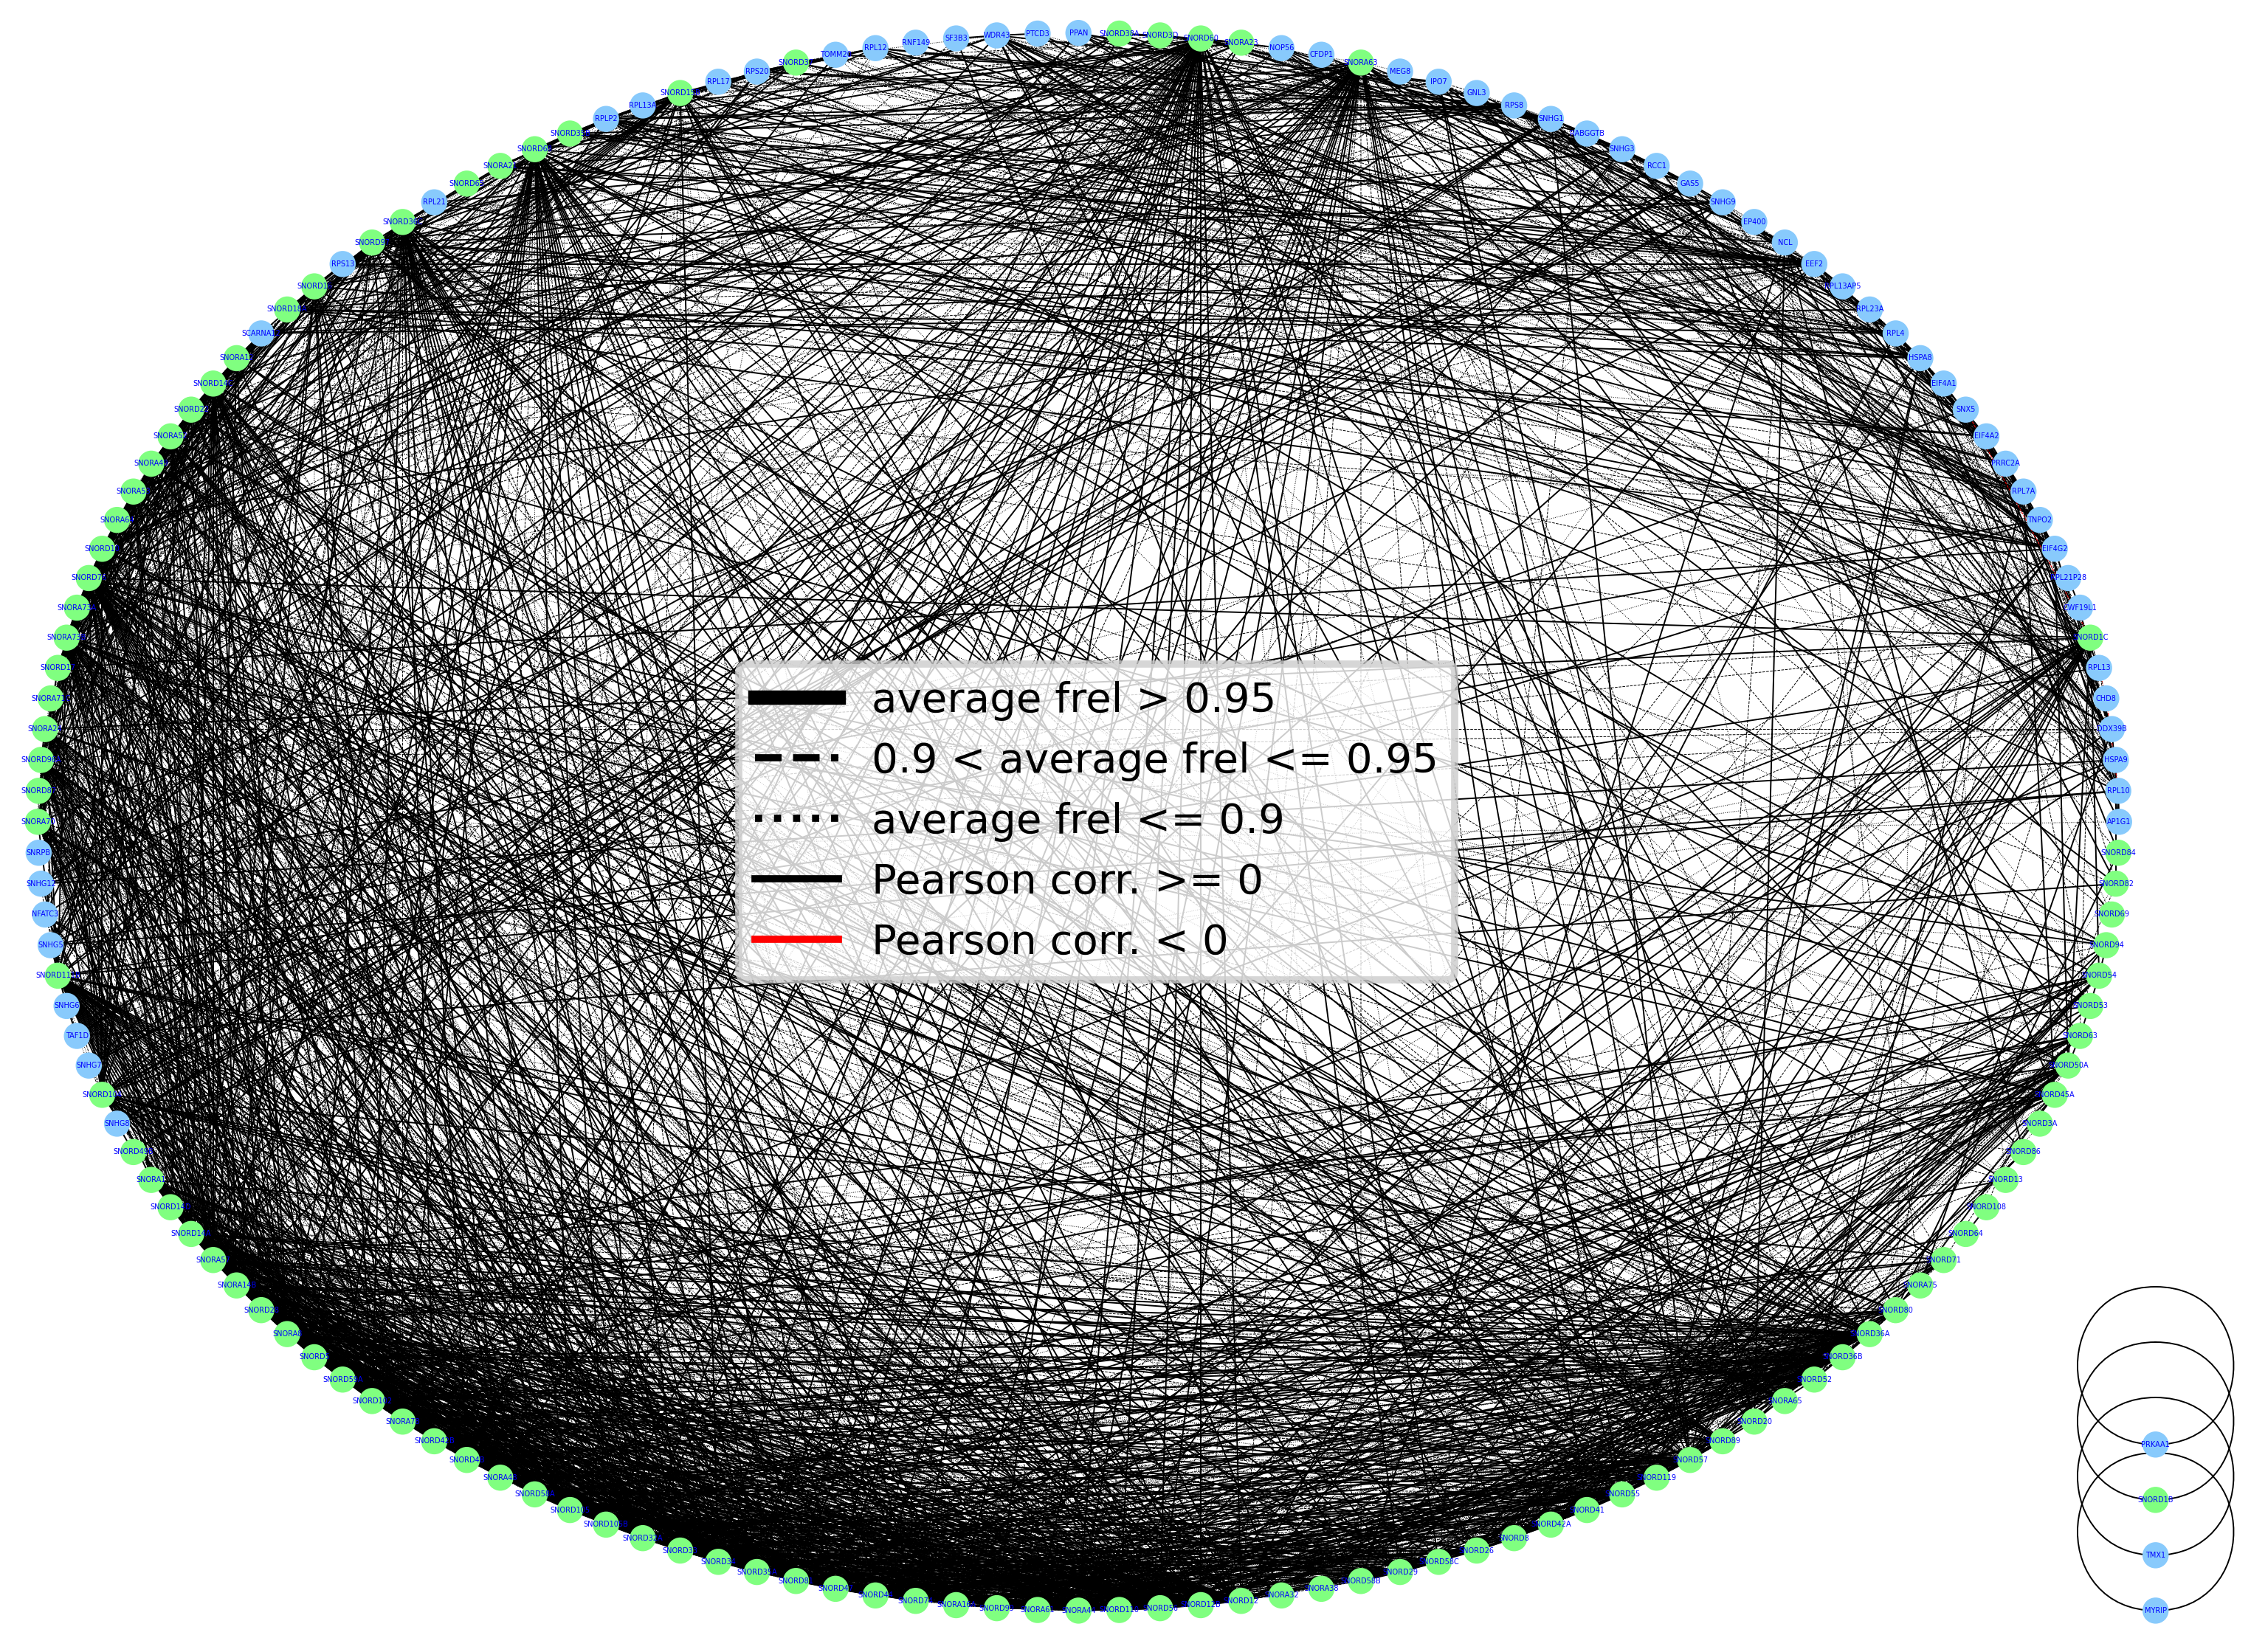
\includegraphics[width=20cm]{images/Complete_Graph_Circular.png}}
    \caption{Circular variant of the complete network graph with ignored edges between isoforms of the same gene - 0.85 threshold}\label{fig:circ_graph_ignored}
\end{figure}

\begin{figure}[!ht]
    \centering
    \rotatebox[origin=c]{90}{\includegraphics[width=20cm]{images/Complete_Graph_0_5.png}}
    \caption{Core network graph with ignored edges between isoforms of the same gene - 0.5 threshold}\label{fig:comp_graph_ignored_0_5}
\end{figure}

\begin{figure}[!ht]
    \centering
    \rotatebox[origin=c]{90}{\includegraphics[width=20cm]{images/Core_Graph.png}}
    \caption{Core network graph with ignored edges between isoforms of the same gene - 0.85 threshold}\label{fig:core_graph_ignored}
\end{figure}

\clearpage
\newpage

\subsection{Differential gene expression analysis}
\begin{figure}[!ht]
    \centering
    \includegraphics[width=0.8\textwidth]{images/DE/pvalueDE.jpg}
    \caption{Distribution of adjusted p-value.}
    \label{fig:pvalueDE}
\end{figure}

\begin{figure}[!ht]
    \centering
    \includegraphics[width=.8\textwidth]{images/DE/volcano1DE.jpg}
    \caption{volcano plot Basal VS Her2}
    \label{fig:volcano1DE_copy}
\end{figure}

\begin{figure}
    \centering
    \includegraphics[width=.8\textwidth]{images/DE/volcano2DE.jpg}
    \caption{volcano plot Control VS Basal}
    \label{fig:volcano2DE}
\end{figure}

\begin{figure}
    \centering
    \includegraphics[width=.8\textwidth]{images/DE/volcano3DE.jpg}
    \caption{volcano plot HER2 VS Luminal A}
    \label{fig:volcano3DE}
\end{figure}

\begin{figure}
    \centering
    \includegraphics[width=.8\textwidth]{images/DE/volcano4DE.jpg}
    \caption{volcano plot Luminal A VS Luminal B}
    \label{fig:volcano4DE}
\end{figure}

\begin{figure}
    \centering
    \includegraphics[width=.8\textwidth]{images/DE/volcano5DE.jpg}
    \caption{volcano plot Luminal B VS Control}
    \label{fig:volcano5DE}
\end{figure}

\begin{figure}
    \centering
    \includegraphics[width=0.8\textwidth]{images/DE/Venn_Up_and_down.jpg}
    \caption{Venn diagram showing both upregulated and downregulated genes.}
    \label{fig:VennDE_copy}
\end{figure}

\begin{figure}
    \centering
    \includegraphics[width=0.8\textwidth]{images/DE/Venn_up.jpg}
    \caption{Venn diagram showing the upregulated genes.}
    \label{fig:Venn_up_DE}
\end{figure}

\begin{figure}
    \centering
    \includegraphics[width=0.8\textwidth]{images/DE/Venn_down.jpg}
    \caption{Venn diagram showing the downregulated genes.}
    \label{fig:Venn_down_DE}
\end{figure}

\begin{figure}
    \centering
    \includegraphics[width=0.8\textwidth]{images/DE/boxplot_DE.jpg}
    \caption{Boxplot with the intensity distributions of the 
individual arrays.}
    \label{fig:boxplotDE}
\end{figure}

%\begin{figure}
%    \centering
%    \includegraphics[width=0.8\textwidth]{images/DE/2022-12-12 10.44.15.jpg}
%    \caption{Caption}
%    \label{fig:graph_DE}
%\end{figure}

\newpage

 
% you can choose not to have a title for an appendix
% if you want by leaving the argument blank
%\section{}


\end{document}

%--------------------------------------------------------------------------------------------------------------

%ROBA DI BACKUP
%SNORA1, SNORA12, SNORA14B, SNORA16A, SNORA21, SNORA23, SNORA24, SNORA32, SNORA38, SNORA44, SNORA48, SNORA49, SNORA52, SNORA53, SNORA57, SNORA61, SNORA63, SNORA64, SNORA65, SNORA70, SNORA71C, SNORA73A, SNORA73B, SNORA75, SNORA78, SNORA8, SNORD10, SNORD102, SNORD104, SNORD105, SNORD105B, SNORD108, SNORD110, SNORD111B, SNORD113-3, SNORD113-4, SNORD114-1, SNORD114-13, SNORD114-14, SNORD114-19, SNORD114-20, SNORD114-21, SNORD115-23, SNORD115-32, SNORD116-13, SNORD119, SNORD12, SNORD12B, SNORD13, SNORD14A, SNORD14C, SNORD14D, SNORD15B, SNORD16, SNORD17, SNORD18A, SNORD1B, SNORD20, SNORD22, SNORD26, SNORD28, SNORD29, SNORD32A, SNORD33, SNORD34, SNORD35A, SNORD36A, SNORD36B, SNORD38A, SNORD3A, SNORD3D, SNORD41, SNORD42A, SNORD42B, SNORD44, SNORD45A, SNORD47, SNORD49B, SNORD4B, SNORD5, SNORD50A, SNORD52, SNORD53, SNORD54, SNORD55, SNORD56, SNORD57, SNORD58A, SNORD58C, SNORD59A, SNORD60, SNORD63, SNORD64, SNORD65, SNORD68, SNORD69, SNORD71, SNORD74, SNORD76, SNORD8, SNORD81, SNORD82, SNORD84, SNORD86, SNORD87, SNORD89, SNORD94, SNORD96A, SNORD97, SNORD99.

%TMX1, ZFAS1, CDKN2B-AS1, CWF19L1, EIF4A1, EP400, HIF1A-AS2, MEG8, NOP56, RACK1, RPL13A, RPS13, SCARNA12, SNHG12, SNHG20, SNHG5, SNHG6, SNHG7, SNHG8.


%\begin{tabular}{cc|ccccc}
%\multicolumn{2}{c}{}
%            &   \multicolumn{2}{c}{Truth} \\
%    &       &   Basal &   HER &     L. A &   L. B &   Normal              \\ 
%    \cline{2-7}
%\multirow{5}{*}{\rotatebox[origin=c]{90}{Predicted}}
%    & Basal   & 0   & 0 & 0& 0& 0                 \\
%    & HER    & 0    & 0 & 0& 0& 0               \\ 
%    & L. A    & 0    & 0 & 0& 0& 0               \\ 
%    & L. B    & 0    & 0 & 0& 0& 0               \\ 
%    & Normal    & 0    & 0 & 0& 0& 0               \\ 
%    \cline{2-7}
%    \end{tabular}